\documentclass[tikz, border = 2pt]{standalone}

%---------------------------------------------------------------------------%
% PACKAGES                                                                  %
%---------------------------------------------------------------------------%

%----- MATH
%---------------------------------------------------------------------------%
\usepackage{amsmath, amssymb}

%----- FIGURES
%---------------------------------------------------------------------------%
\usepackage{color}
\usepackage{pgfplots}
\pgfplotsset{compat=1.13}

%---------------------------------------------------------------------------%
%                                MINES COLORS                               %
%---------------------------------------------------------------------------%

%---------- OFFICIAL COLORS
\definecolor{MPTblue}{RGB}{0,94,158}

\begin{document}

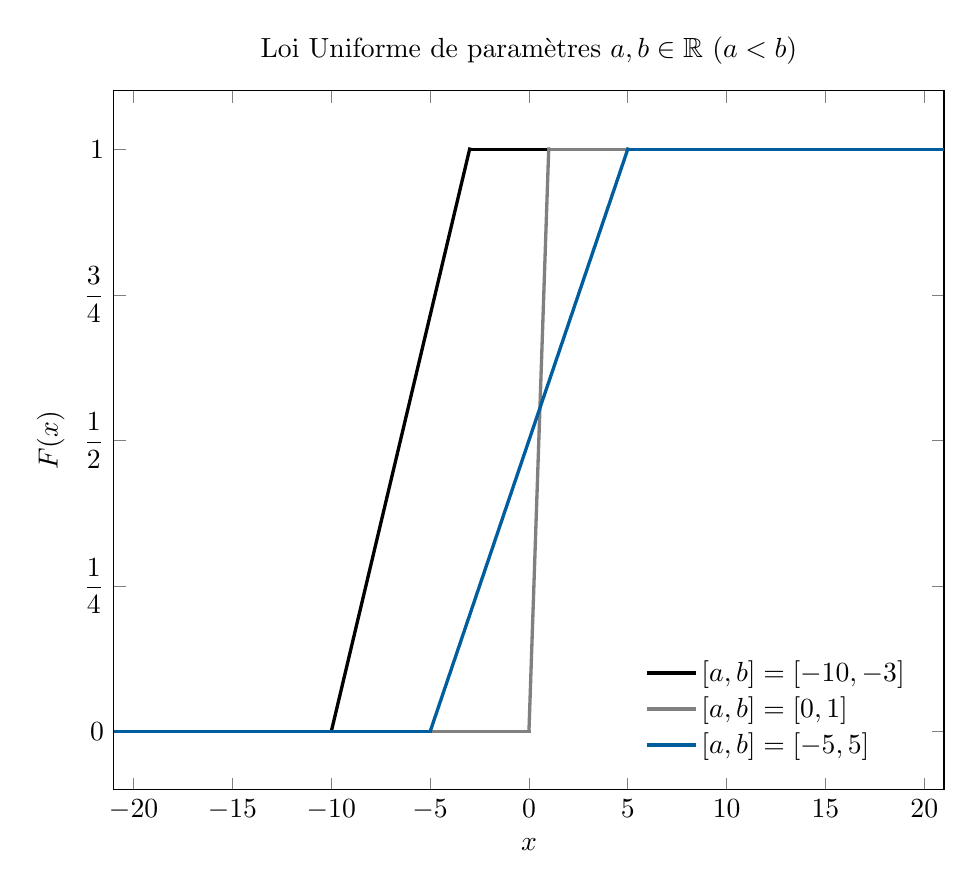
\begin{tikzpicture}
\begin{axis}[width = \textwidth,
title style = {align = center},
title={Loi Uniforme de param\`etres $a,b \in \mathbb{R}$ ($a<b$)},
xlabel={$x$},
ylabel={$F(x)$},
legend pos = south east,
legend style = {draw=none},
legend cell align = left,
xmin = -21,
xmax = 21,
ytick = {0,0.25,0.5,0.75,1},
yticklabels = {$0$, $\dfrac{1}{4}$, $\dfrac{1}{2}$, $\dfrac{3}{4}$, $1$},
ylabel near ticks,
domain = -21:21
]
\addplot[black, very thick, samples = 2, domain = -10:-3, shorten >=-0.15ex] {(x+10)/7};
\addplot[black, very thick, samples = 2, domain = -21:-10, shorten >=-0.15ex, forget plot] {0};
\addplot[black, very thick, samples = 2, domain = -3:21, forget plot] {1};
%
\addplot[black!50, very thick, samples = 2, domain = 0:1, shorten >=-0.15ex] {x};
\addplot[black!50, very thick, samples = 2, domain = -21:0, shorten >=-0.15ex, forget plot] {0};
\addplot[black!50, very thick, samples = 2, domain = 1:21, forget plot] {1};
%
\addplot[MPTblue, very thick, samples = 2, domain = -5:5, shorten >=-0.15ex] {(x+5)/10};
\addplot[MPTblue, very thick, samples = 2, domain = -21:-5, shorten >=-0.15ex, forget plot] {0};
\addplot[MPTblue, very thick, samples = 2, domain = 5:21, forget plot] {1};

%
\legend{{$[a,b] = [-10,-3]$}, {$[a,b] = [0,1]$}, {$[a,b] = [-5,5]$}}
\end{axis}
\end{tikzpicture}

\end{document}